% Options for packages loaded elsewhere
\PassOptionsToPackage{unicode}{hyperref}
\PassOptionsToPackage{hyphens}{url}
%
\documentclass[
]{article}
\usepackage{amsmath,amssymb}
\usepackage{lmodern}
\usepackage{iftex}
\ifPDFTeX
  \usepackage[T1]{fontenc}
  \usepackage[utf8]{inputenc}
  \usepackage{textcomp} % provide euro and other symbols
\else % if luatex or xetex
  \usepackage{unicode-math}
  \defaultfontfeatures{Scale=MatchLowercase}
  \defaultfontfeatures[\rmfamily]{Ligatures=TeX,Scale=1}
\fi
% Use upquote if available, for straight quotes in verbatim environments
\IfFileExists{upquote.sty}{\usepackage{upquote}}{}
\IfFileExists{microtype.sty}{% use microtype if available
  \usepackage[]{microtype}
  \UseMicrotypeSet[protrusion]{basicmath} % disable protrusion for tt fonts
}{}
\makeatletter
\@ifundefined{KOMAClassName}{% if non-KOMA class
  \IfFileExists{parskip.sty}{%
    \usepackage{parskip}
  }{% else
    \setlength{\parindent}{0pt}
    \setlength{\parskip}{6pt plus 2pt minus 1pt}}
}{% if KOMA class
  \KOMAoptions{parskip=half}}
\makeatother
\usepackage{xcolor}
\IfFileExists{xurl.sty}{\usepackage{xurl}}{} % add URL line breaks if available
\IfFileExists{bookmark.sty}{\usepackage{bookmark}}{\usepackage{hyperref}}
\hypersetup{
  hidelinks,
  pdfcreator={LaTeX via pandoc}}
\urlstyle{same} % disable monospaced font for URLs
\usepackage[margin=1in]{geometry}
\usepackage{graphicx}
\makeatletter
\def\maxwidth{\ifdim\Gin@nat@width>\linewidth\linewidth\else\Gin@nat@width\fi}
\def\maxheight{\ifdim\Gin@nat@height>\textheight\textheight\else\Gin@nat@height\fi}
\makeatother
% Scale images if necessary, so that they will not overflow the page
% margins by default, and it is still possible to overwrite the defaults
% using explicit options in \includegraphics[width, height, ...]{}
\setkeys{Gin}{width=\maxwidth,height=\maxheight,keepaspectratio}
% Set default figure placement to htbp
\makeatletter
\def\fps@figure{htbp}
\makeatother
\setlength{\emergencystretch}{3em} % prevent overfull lines
\providecommand{\tightlist}{%
  \setlength{\itemsep}{0pt}\setlength{\parskip}{0pt}}
\setcounter{secnumdepth}{-\maxdimen} % remove section numbering
\newlength{\cslhangindent}
\setlength{\cslhangindent}{1.5em}
\newlength{\csllabelwidth}
\setlength{\csllabelwidth}{3em}
\newlength{\cslentryspacingunit} % times entry-spacing
\setlength{\cslentryspacingunit}{\parskip}
\newenvironment{CSLReferences}[2] % #1 hanging-ident, #2 entry spacing
 {% don't indent paragraphs
  \setlength{\parindent}{0pt}
  % turn on hanging indent if param 1 is 1
  \ifodd #1
  \let\oldpar\par
  \def\par{\hangindent=\cslhangindent\oldpar}
  \fi
  % set entry spacing
  \setlength{\parskip}{#2\cslentryspacingunit}
 }%
 {}
\usepackage{calc}
\newcommand{\CSLBlock}[1]{#1\hfill\break}
\newcommand{\CSLLeftMargin}[1]{\parbox[t]{\csllabelwidth}{#1}}
\newcommand{\CSLRightInline}[1]{\parbox[t]{\linewidth - \csllabelwidth}{#1}\break}
\newcommand{\CSLIndent}[1]{\hspace{\cslhangindent}#1}
\usepackage{booktabs}
\usepackage{longtable}
\usepackage{array}
\usepackage{multirow}
\usepackage{wrapfig}
\usepackage{float}
\usepackage{colortbl}
\usepackage{pdflscape}
\usepackage{tabu}
\usepackage{threeparttable}
\usepackage{threeparttablex}
\usepackage[normalem]{ulem}
\usepackage{makecell}
\usepackage{xcolor}
\ifLuaTeX
  \usepackage{selnolig}  % disable illegal ligatures
\fi

\author{}
\date{\vspace{-2.5em}}

\begin{document}

{
\setcounter{tocdepth}{2}
\tableofcontents
}
\newpage

LMA responses of understory plants to artificial light at night

\[ \]

Cong Zhou\textsuperscript{1,2}, Akihiro Nakamura\textsuperscript{1},
Masatoshi Katabuchi\textsuperscript{1},

\[ \]

\textsuperscript{1} CAS Key Laboratory of Tropical Forest Ecology,
Xishuangbanna Tropical Botanical Garden, Chinese Academy of Sciences,
Menglun, Yunnan 666303, China

\textsuperscript{2} University of Chinese Academy of Sciences, Beijing
100049, China

\[ \]

\textbf{Corresponding Authors}:

Masatoshi Katabuchi

E-mail:
\href{mailto:mattocci27@gmail.com}{\nolinkurl{mattocci27@gmail.com}}

\[ \]

Manuscript received \_\_\_\_\_\_\_; revision accepted \_\_\_\_\_\_\_.

\textbf{Running title}:

\newpage

\hypertarget{abstract}{%
\section{ABSTRACT}\label{abstract}}

\textbf{PREMISE:} Artificial light at night (ALAN),

\textbf{METHODS:}

\textbf{RESULTS:}

\textbf{CONCLUSIONS:}

\textbf{KEY WORDS} light pollution, leaf mass per area (LMA), leaf
punch, Artificial light at night (ALAN)

\hypertarget{introduction}{%
\section{INTRODUCTION}\label{introduction}}

Light pollution caused by artificial light at night (ALAN) has disturbed
ecological processes since the start of 20th century
(\protect\hyperlink{ref-Bennie2016}{Bennie et al. 2016};
\protect\hyperlink{ref-Longcore2004}{Longcore and Rich 2004};
\protect\hyperlink{ref-Gaston2013}{Gaston et al. 2013}). So far,
artificial light at night extends both in intensity covered a large
illuminance range from the degree hard to detect to almost daylight and
in extent covered more and more World's terrestrial surfaces
(\protect\hyperlink{ref-Bennie2016}{Bennie et al. 2016};
\protect\hyperlink{ref-Falchi2016}{2016}). ALAN influences behavior or
physiology broad ranges of taxonomic groups including mammals, birds,
reptiles, amphibians, fishes, invertebrates, and plants
(\protect\hyperlink{ref-Rich2006}{Rich and Longcore 2006}). For example,
ALAN attracts insects \ldots. so as an important bringer to drive
insects population decline
(\protect\hyperlink{ref-Boyes2021}{\textbf{Boyes2021?}};
\protect\hyperlink{ref-Owens2020}{Owens et al. 2020}). Although many
studies have focused on how ALAN change the behavior of animals (ref),
its influence on plants has also received attentions {[}Speißer, Liu,
and van Kleunen (\protect\hyperlink{ref-Speisser2021a}{2021}); Liu2022
Matthew effect{]}. A recent studies experimentally showed that ALAN
increases biomass of herbaceous plants, which suggests ALAN can work as
the light resources for plant growth
(\protect\hyperlink{ref-Speisser2021a}{Speißer, Liu, and van Kleunen
2021}). However, few studies have examined the effects of ALAN on plant
functional traits in conditions close to their natural environment.

ALAN might directly affect plant leaf functional traits because ALAN
could work as the light resources. Although LMA is driven by inherent
genetic mechanisms
(\protect\hyperlink{ref-Asner2011}{\textbf{Asner2011?}}), environmental
stresses (temperature, water and light) also shapes LMA. Actually,
plants could sense light through photorecpetors which allows the plant
to respond to four parameters of their light environment: light spectral
quality, light intensity, light direction, and light duration
(\protect\hyperlink{ref-Paik2019}{Paik and Huq 2019};
\protect\hyperlink{ref-Rich2006}{Rich and Longcore 2006}).
(\protect\hyperlink{ref-Terashima2006}{\textbf{Terashima2006?}}) showed
that the light-saturated rate of leaf photosynthesis per unit area
(\(P_max\)) is highly correlated with leaf structural parameters such as
leaf thickness, leaf mass per area, mesophyll surface area(\(S_mes\)),
and chloroplast surface area (\(S_c\)), and sun leaves are thicker than
shade leaves exactly as the height of the palisade tissue in sun leaves
is greater than that in shade leaves. For individual species, LMA was
proportional with species distributions along the insolation gradient,
and was significantly higher in evergreen versus deciduous species
(\protect\hyperlink{ref-Ackerly2002}{\textbf{Ackerly2002?}};
\protect\hyperlink{ref-Onoda2008}{\textbf{Onoda2008?}};
\protect\hyperlink{ref-Niinemets2004}{\textbf{Niinemets2004?}}). And
among a local community,
(\protect\hyperlink{ref-Ackerly2002}{\textbf{Ackerly2002?}})
demonstrated the average values of LMA significantly increased with
increasing potential diurnal insolation(PDI). Here, ALAN could be
considered as a conduct of prolonging light duration to plants so plants
LMA could increase with that.

On the other hand, ALAN might indirectly affect plant leaf functional
traits because ALAN has a potential to change soil environmental
conditions by attracting insects. Many kinds of insects orient
themselves by maintaining a constant angle to light rays and are
attracted by light {[}positive phototaxis?
(\protect\hyperlink{ref-Baker1978}{Baker and Sadovy 1978};
\protect\hyperlink{ref-Sotthibandhu1979}{Sotthibandhu and Baker
1979}){]}. Previous studies showed that 30--40\% of insects die soon
after approaching street lamps for collision, overheating, dehydration,
or predation (\protect\hyperlink{ref-Minnaar2015}{Minnaar et al. 2015};
\protect\hyperlink{ref-Owens2018}{Owens and Lewis 2018}). Since nitrogen
(N) and phosphorus (P) are the nutrients most frequently limiting
primary productivity in forest ecosystems (refs), dead insects killed by
ALAN could be important nutrient input for soil nutrient. Soil
resources, especially N and P availability, are known to affect leaf
mass per area (LAM) and leaf N and P contents (refs), and those effects
are known to be opposite to the effects of light (refs) (e.g., strong
light increase LMA but high N availability decrease LMA).

Here we report the results of a 2-year ALAN experiment in forest
understory to simulate light pollution. Two species were chosen in this
experiment representing sun species and shade species respectively to
test whether different responds would show between them. We predicted
that ALAN would bring effect to understory both aboveground as direct
light supplementary and undergound as indirect soil nutrients
supplementary. We also predicted that canopy-openness and its
interaction with artificial light at night would show weaker impaction
in this experiment.

\hypertarget{materials-and-methods}{%
\section{MATERIALS AND METHODS}\label{materials-and-methods}}

\emph{experimental setup}

The field experiment was located within the Xishuangbanna Tropical
Botanical Garden (XTBG),China in rubber tree forest (N21°54' E101°16')
where we totally set 5 plots and selected 2 plots for this this after
field investiation. LED (10w) is used to create an artificial light
environment in all plots at night.(fig.~) The LED system includes 6
components. A metal box with an opening is used as a rainproof protector
which is attached to a tree at around 1.2 m from the ground. A
rechargeable lithium battery (12v/30Ah) and an electric timer controls
the timing and duration of the LED light operation at night. An electric
wire was used to connect battery and LED which was hanging from a tree
branch with a lampshade at approximately 2 m from the ground. Then the
LED would work automatically from 8 pm to 5 am every day. This
experiment started from 2019 November, and samples were collected on
2021 November.

\emph{Species Selection}

Considering the understory condition (enough mature individual numbers,
distribution of individuals) and species specificity(it should be
evergreen species, and not be the nitrogen fix plants like Leguminosae)
of each plot, finally two species respectively in two plots were chosen
for our study, \emph{Colocasia gigantea (Blume) Hook. f.} representing
shade species and \emph{Melastoma candidum D. Don} for sun species.

\emph{Measurements}

We measured the horizontal distance and geographic orientation of each
individual away from the LED using tape measure representing the
relative effects of ALAN. Canopy openness was selected to be on behalf
of day light, which photographed by Nikon COOLPIX4500 with fish-eye lens
(Nikon FC-e8) then measured using R package
\emph{LeafArea}(\protect\hyperlink{ref-Katabuchi2015}{\textbf{Katabuchi2015?}}).
For leaf mass per area (LMA), we use leaf disc (10mm\^{}2) punched from
leaf avoiding vein and leaf margin instead of whole-leaf to calculate
LMA value.(fig.~)

\emph{Data Analysis}

To analyze the effects of ALAN, daylight's effect, and their interaction
on both \emph{Melastoma candidum D. Don} and \emph{Colocasia gigantea
(Blume) Hook. f.}, We fitted a Bayesian linear mixed-effets model for
each species using `rstan' package in R. Leaf mass per area (LMA) of
each leaf of each individual was the response variable. Distance from
the ALAN of each individual was transformed by log and reciprocal for
both the accumulation of insects and the intensity of ALAN fade away
from distance. We conducted individual as a random effect for each
species on our model, for the non-independence of individuals of the
same species. All statistical analyses were conducted in R version 4.1.2
(\protect\hyperlink{ref-RCoreTeam2021}{\textbf{RCoreTeam2021?}}). ** how
to cite R? **

\hypertarget{results}{%
\section{RESULTS}\label{results}}

For species \emph{Colocasia gigantea (Blume) Hook. f.}, both the effcts
of ALAN and daylight were significant, while species \emph{Melastoma
candidum D. Don} showed no significance. Artificial light at night drove
the averaged individual LMA value decrease for species \emph{Colocasia
gigantea (Blume) Hook. f.} (mean: -0.1043) and for species
\emph{Melastoma candidum D. Don} (mean: -0.0422) although not
significant. Both species showed no significance on the interaction of
the effects of ALAN and daylight. (Table 1.)

\hypertarget{discussion}{%
\section{DISCUSSION}\label{discussion}}

Although it has been demonstrated that LMA increase with
insolation{[}{]}, our research shows the artificial light situation
could make differences. Actually, artificial light at night exerts an
influence on the physiological processes of understory by multi-approach
both aboveground and undergound. For aboveground part, artificial light
at night change the light environments of plants including light
duration, light intensity and light spectral quality. For underground
part, artificial light at night indirectly changed the soil nutrients
conditions especially as an important nitrogen supplementary. So the
response results of understory could vary according to the species
specificity{[}{]} and artificial light resource{[}{]}.

There was research showed that plants' biomass would increase under
artificial light{[}{]}, our study showed the change part of biomass
could be channelled into mixed results. Further more, adequate tests of
the influence of artificial light at night on understory will entail
more experimental work under field conditions. Controlling experiment
probably tend to underestimate the environmental heterogeneity and
species interaction, because many irreplaceable features of field
conditions, such as subtle nutrients change, herbivores and competitors
are usually absent. Hence the general pattern how understory species
responds to artificial light at night remains unknown. In future work,
diverse artificial light resource in light spectral quality and light
intensity is need to simulate multi-situation of artificial light. And
if possible, long term field experiment combining with controlling
experiment approaching to plants natural growth situation will figure
out the generalized patterns.

In conclusion, our study showed the LMA of some understory species would
decrease with artificial light at night. The effects of artificial light
at night consists of aboveground part directly as light resource and
undergound part indirectly as soil nutrients. Still, more studies are
needed to reveal the comprehensive effcts, from plant physiology to
plant community. Nevertheless, the negative effct of artificial light at
night on understory species indicates that increments of artificial
light at night might bring about a physiological suppression to those
understory plants.

Ignoring the effect of artificial light at night to multilevel
ecological processes is self-deception, hence more and more research
would be carried through about this important topic
(\protect\hyperlink{ref-Davies2018}{Davies and Smyth 2018}).

\hypertarget{ackonwlegements}{%
\section{ACKONWLEGEMENTS}\label{ackonwlegements}}

\hypertarget{author-contributions}{%
\section{AUTHOR CONTRIBUTIONS}\label{author-contributions}}

MK and CZ conceived the study; CZ collected data and performed the
analysis with MK together; all authors contributed to revisions.

\hypertarget{data-availability-statement}{%
\section{DATA AVAILABILITY
STATEMENT}\label{data-availability-statement}}

\hypertarget{supporting-information}{%
\section{SUPPORTING INFORMATION}\label{supporting-information}}

\hypertarget{literature-cited}{%
\section{LITERATURE CITED}\label{literature-cited}}

\hypertarget{refs}{}
\begin{CSLReferences}{1}{0}
\leavevmode\vadjust pre{\hypertarget{ref-Baker1978}{}}%
Baker, R. Robin, and Yvonne Sadovy. 1978. {``The Distance and Nature of
the Light-Trap Response of Moths.''} \emph{Nature} 276 (December):
818--21. \url{https://doi.org/10.1038/276818a0}.

\leavevmode\vadjust pre{\hypertarget{ref-Bennie2016}{}}%
Bennie, Jonathan, Thomas W. Davies, David Cruse, and Kevin J. Gaston.
2016. {``Ecological Effects of Artificial Light at Night on Wild
Plants.''} \emph{Journal of Ecology} 104 (3): 611--20.
\url{https://doi.org/10.1111/1365-2745.12551}.

\leavevmode\vadjust pre{\hypertarget{ref-Davies2018}{}}%
Davies, Thomas W., and Tim Smyth. 2018. {``Why Artificial Light at Night
Should Be a Focus for Global Change Research in the 21st Century.''}
\emph{Global Change Biology} 24 (3): 872--82.
\url{https://doi.org/10.1111/gcb.13927}.

\leavevmode\vadjust pre{\hypertarget{ref-Falchi2016}{}}%
Falchi. 2016. {``The New World Atlas of Artificial Night Sky
Brightness.''} https://www.science.org/doi/10.1126/sciadv.1600377.
\url{https://doi.org/10.1126/sciadv.1600377}.

\leavevmode\vadjust pre{\hypertarget{ref-Gaston2013}{}}%
Gaston, Kevin J., Jonathan Bennie, Thomas W. Davies, and John Hopkins.
2013. {``The Ecological Impacts of Nighttime Light Pollution: A
Mechanistic Appraisal.''} \emph{Biological Reviews} 88 (4): 912--27.
\url{https://doi.org/10.1111/brv.12036}.

\leavevmode\vadjust pre{\hypertarget{ref-Longcore2004}{}}%
Longcore, Travis, and Catherine Rich. 2004. {``Ecological Light
Pollution.''} \emph{Frontiers in Ecology and the Environment} 2 (4):
191--98.
\url{https://doi.org/10.1890/1540-9295(2004)002\%5B0191:ELP\%5D2.0.CO;2}.

\leavevmode\vadjust pre{\hypertarget{ref-Minnaar2015}{}}%
Minnaar, Corneile, Justin G. Boyles, Ingrid A. Minnaar, Catherine L.
Sole, and Andrew E. McKechnie. 2015. {``Stacking the Odds: Light
Pollution May Shift the Balance in an Ancient Predator\textendash prey
Arms Race.''} \emph{Journal of Applied Ecology} 52 (2): 522--31.
\url{https://doi.org/10.1111/1365-2664.12381}.

\leavevmode\vadjust pre{\hypertarget{ref-Owens2020}{}}%
Owens, Avalon C. S., Précillia Cochard, Joanna Durrant, Bridgette
Farnworth, Elizabeth K. Perkin, and Brett Seymoure. 2020. {``Light
Pollution Is a Driver of Insect Declines.''} \emph{Biological
Conservation} 241 (January): 108259.
\url{https://doi.org/10.1016/j.biocon.2019.108259}.

\leavevmode\vadjust pre{\hypertarget{ref-Owens2018}{}}%
Owens, Avalon C. S., and Sara M. Lewis. 2018. {``The Impact of
Artificial Light at Night on Nocturnal Insects: {A} Review and
Synthesis.''} \emph{Ecology and Evolution} 8 (22): 11337--58.
\url{https://doi.org/10.1002/ece3.4557}.

\leavevmode\vadjust pre{\hypertarget{ref-Paik2019}{}}%
Paik, Inyup, and Enamul Huq. 2019. {``Plant Photoreceptors:
{Multi-functional} Sensory Proteins and Their Signaling Networks.''}
\emph{Seminars in Cell \& Developmental Biology} 92 (August): 114--21.
\url{https://doi.org/10.1016/j.semcdb.2019.03.007}.

\leavevmode\vadjust pre{\hypertarget{ref-Rich2006}{}}%
Rich, Catherine, and Travis Longcore. 2006. {``Ecological Consequences
of Artificial Night Lighting.''} In.

\leavevmode\vadjust pre{\hypertarget{ref-Sotthibandhu1979}{}}%
Sotthibandhu, S., and R. R. Baker. 1979. {``Celestial Orientation by the
Large Yellow Underwing Moth, {Noctua} Pronuba {L}.''} \emph{Animal
Behaviour} 27 (August): 786--800.
\url{https://doi.org/10.1016/0003-3472(79)90015-0}.

\leavevmode\vadjust pre{\hypertarget{ref-Speisser2021a}{}}%
Speißer, Benedikt, Yanjie Liu, and Mark van Kleunen. 2021. {``Biomass
Responses of Widely and Less-Widely Naturalized Alien Plants to
Artificial Light at Night.''} \emph{Journal of Ecology} 109 (4):
1819--27. \url{https://doi.org/10.1111/1365-2745.13607}.

\end{CSLReferences}

\newpage

\textbf{Fig. 1.} The distribution of individuals around the ALAN and the
illustration of the experiment setup. (). The locations of the
artificial-light-at-night plots and relative locations of each
individual, each triangle represents one individual and the size of it
represents the averaged LMA value. () and (). Photographs of the
experiment during the day and night.

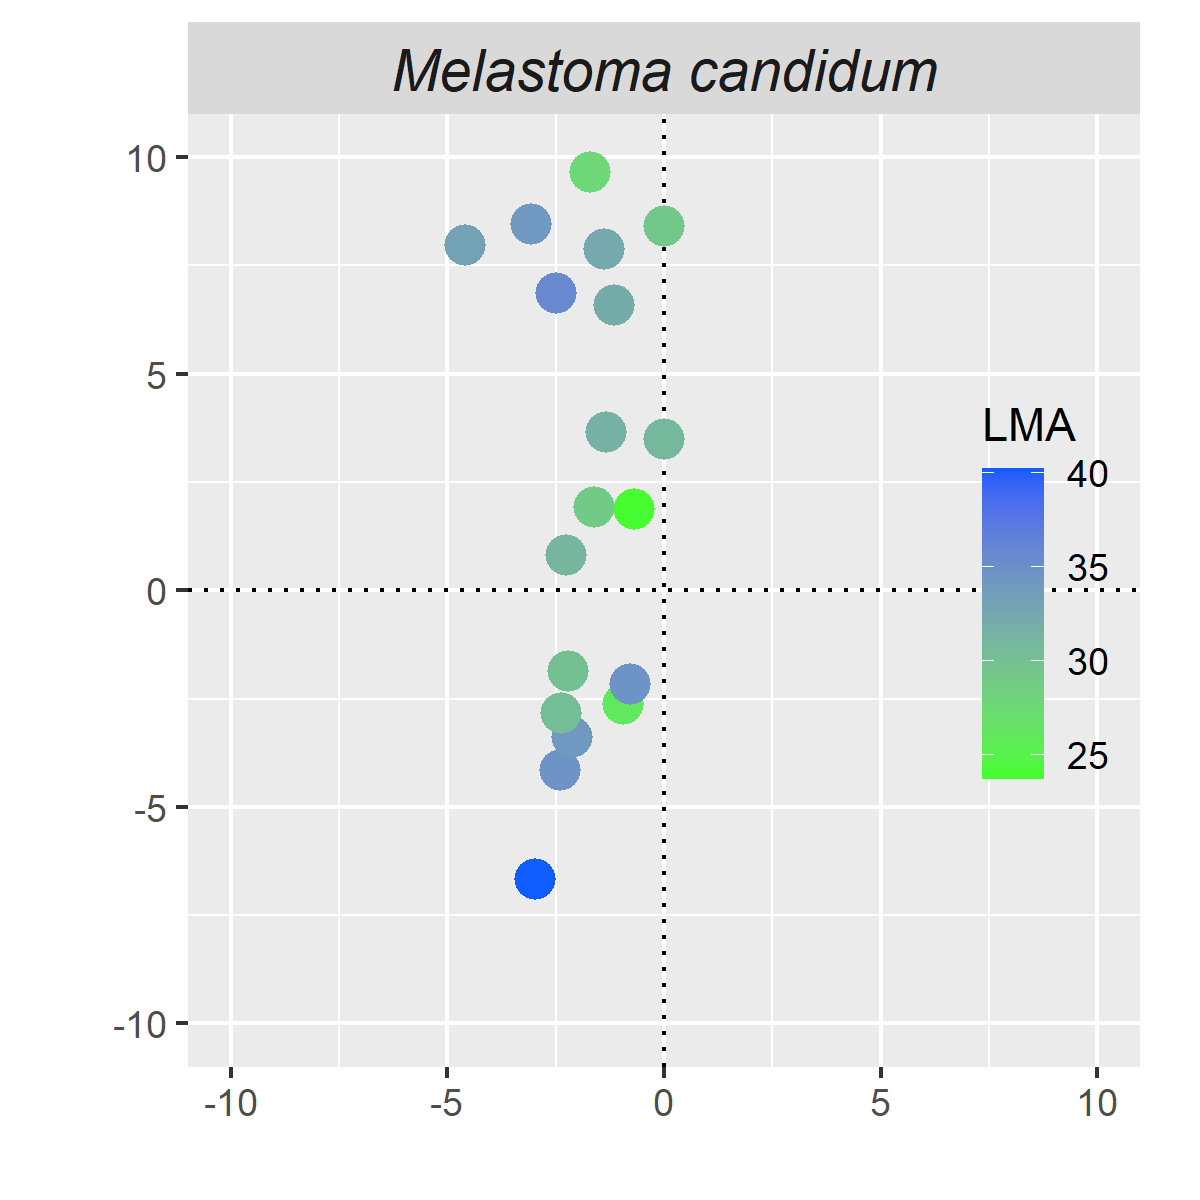
\includegraphics{../light_project/figs/sp1-dis}

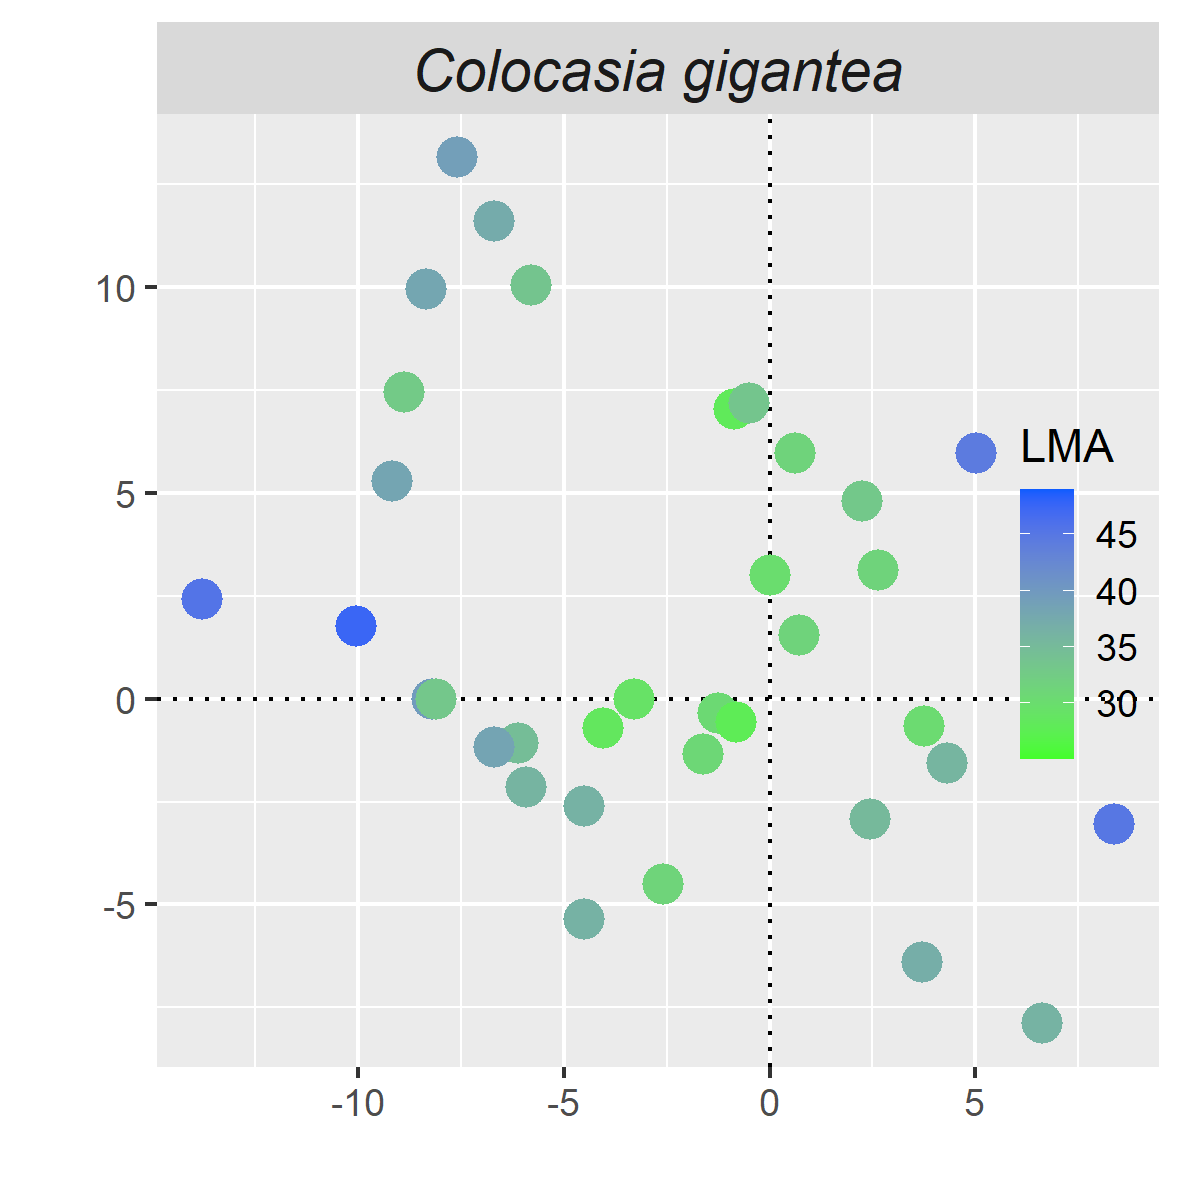
\includegraphics{../light_project/figs/sp2-dis}

\newpage

\#\texttt{\{r\ table,\ echo=FALSE\}\ table\ \textless{}-\ read.csv("../light\_project/data-raw/table.csv")\%\textgreater{}\%\ \ \ kbl(caption\ =\ "Coefficients\ table")\ \%\textgreater{}\%\ \ \ kable\_paper("striped",\ full\_width\ =\ F)\ \%\textgreater{}\%\ \ \ column\_spec(4,\ bold\ =\ c(F,F,F,T,T,F))\ \%\textgreater{}\%\ \ \ pack\_rows("Melastoma\_candidum",\ 1,\ 3)\ \%\textgreater{}\%\ \ \ pack\_rows("Colocasia\_gigantea",\ 4,\ 6)\ table}

\textbf{Table. 1.} Results of Bayesian general linear mixed-effect
models testing the effects of artificial light at night, daylight and
interaction on experimental species. Significant effects (p \textless{}
0.05) are in bold.

\newpage

\end{document}
